\documentclass[journal]{IEEEtran}
\usepackage[T1]{fontenc}
\usepackage[utf8]{inputenc}
\usepackage[polish]{babel}
\usepackage{graphicx}
\usepackage{subcaption}
\pagestyle{plain}
\setlength{\parskip}{0.7em}  
\setlength{\parindent}{15pt}


\ifCLASSINFOpdf
  
\else
 
\fi





% correct bad hyphenation here
\hyphenation{op-tical net-works semi-conduc-tor}


\begin{document}

\title{Analiza zmienności rytmu serca z wykorzystaniem urządzeń mobilnych}
\author{
    J. Bancerewicz, J. Kotłowski, O. Lozovyy, J. Morawska, M. Rzęsa\\
    \textit{Politechnika Gdańska}\\
    \textit{Wydział Elektroniki, Telekomunikacji i Informatyki}
}


% The paper headers
\markboth{}%
{Shell \MakeLowercase{\textit{et al.}}: Bare Demo of IEEEtran.cls for IEEE Journals}
\maketitle

\begin{abstract}
W niniejszej pracy przedstawiono metody analizy zmienności rytmu serca na podstawie sygnałów elektrokardiograficznych i fotopletyzmograficznych pozyskiwanych za pomocą urządzeń przenośnych. Opracowano proces przetwarzania zapisów obejmujący tłumienie zakłóceń, wykrywanie pików oraz wyznaczanie interwałów między impulsami w przebiegu fizjologicznym. Detekcję szczytów R w EKG oraz maksimów fali w PPG zrealizowano z wykorzystaniem splotowych i rekurencyjnych sieci neuronowych. Skuteczność modeli oceniono w odniesieniu do klasycznych algorytmów jak i danych referencyjnych. Wyniki wykazały wysoką dokładność identyfikacji pików oraz umożliwiają zastosowanie mobilnych systemów do monitorowania parametrów kardiologicznych w warunkach domowych i podczas aktywności fizycznej.

\textbf{Słowa kluczowe---}zmienność rytmu serca; sygnały biomedyczne; elektrokardiografia; fotopletyzmografia; filtracja sygnałów; splotowe sieci neuronowe; detekcja szczytów; interwał propagacji tętna; algorytm Pan-Tompkins; analiza czasowa.
\end{abstract}


\section{Wstęp}
Zmienność rytmu serca stanowi istotny parametr oceny funkcjonowania układu sercowo-naczyniowego, odzwierciedlający równowagę pomiędzy aktywnością układu współczulnego i przywspółczulnego. Tradycyjne pomiary HRV prowadzone w warunkach klinicznych charakteryzują się wysokim kosztem oraz ograniczonym czasem rejestracji. W ostatnich latach postęp technologiczny w obszarze urządzeń przenośnych oraz sensorów optycznych umożliwił monitorowanie aktywności kardiologicznej w trakcie życia codziennego.

Mobilna akwizycja zapisów elektrokardiograficznych i fotopletyzmograficznych wymaga wysokiej odporności na zakłócenia ruchowe i środowiskowe. Metodologia łącząca cyfrową filtrację sygnałów z sieciami typu CNN i RNN pozwala na automatyczne wykrywanie szczytów R oraz maksimów PPG. Zastosowane podejście wspiera wyznaczanie interwałów RR i IBI, obliczanie wskaźników HRV oraz estymację propagacji tętna w oparciu o zsynchronizowane przebiegi.

Upowszechnienie metod głębokiego uczenia w połączeniu z dostępnością wysokiej jakości danych biomedycznych sprzyjają automatycznej interpretacji sygnałów w warunkach ambulatoryjnych. Istotnymi czynnikami pozostają precyzja detekcji oraz analiza długoterminowa reakcji organizmu na stres, wysiłek i regenerację. Integracja sztucznej inteligencji z systemami przenośnymi wspiera rozwój zdalnej diagnostyki i szczegółowe monitorowanie stanu zdrowia.

\newpage
\section{Techniki filtracji i modelowania sygnałów biomedycznych}
Elektrokardiografia i fotopletyzmografia należą do podstawowych źródeł sygnałów biomedycznych wykorzystywanych w nowoczesnych systemach diagnostycznych i monitorujących. Proces przetwarzania zapisów jest ukierunkowany na uzyskanie wiarygodnych informacji fizjologicznych przy obecności zakłóceń wynikających z ruchu pacjenta, interferencji środowiskowych i ograniczeń sprzętowych. Dominują dwa podejścia: filtrację danych oraz modelowanie wspierane sztuczną inteligencją, które są łączone  dla poprawy dokładności i zwiększenia odporności analizy w warunkach medycznych.

\subsection{Filtracja danych}
Wstępne przetwarzanie przebiegów fizjologicznych opiera się na eliminacji zakłóceń, umożliwiając poprawę stosunku sygnału do szumu. W elektrokardiografii oraz fotopletyzmografii istotną rolę odgrywają niedokładności pomiarowe związane z ruchem, składowe sieciowe o częstotliwości 50/60 Hz oraz dryft linii izoelektrycznej \cite{1}. Filtracja podnosi jakość zapisu, poprawiając dokładność detekcji cech oraz efektywność klasyfikacji.

Do podstawowych metod analizy sygnału należą filtry pasmowoprzepustowe, ograniczające pasmo częstotliwości do wartości charakterystycznych dla badanego przebiegu. Zakres przetwarzania zapisu EKG wynosi 0,5–40 Hz, natomiast PPG ogranicza się do 0,3–8 Hz, odpowiadającego rytmowi serca. W implementacjach cyfrowych wykorzystuje się filtry Butterwortha, Chebysheva, eliptyczne w postaci IIR oraz FIR projektowane metodą okienkową, zapewniające stabilność i liniową charakterystykę fazową \cite{2}. 

Dla sygnałów z zakłóceniami o zmiennych parametrach stosuje się filtry adaptacyjne. Algorytmy LMS i RLS umożliwiają dynamiczną adaptację współczynników układu do charakterystyki zapisu, zwiększając skuteczność tłumienia niestabilności ruchowych oraz interferencji sieciowych. W zastosowaniach medycznych mechanizmy notch zapewniają eliminację składowej 50/60 Hz \cite{3}.

\newpage
Eliminacja artefaktów impulsowych i krótkotrwałych jest realizowana w oparciu o filtry medianowe oraz metody morfologiczne, umożliwiające zachowanie cech diagnostycznych, takich jak załamki QRS \cite{4}. Analiza falkowa oraz techniki Empirical Mode Decomposition i Wavelet Packet Transform zapewniają dekompozycję sygnału na składowe częstotliwościowe oraz selektywne tłumienie szumów przy utrzymaniu struktury pików przebiegu \cite{5}.

W zaawansowanych zastosowaniach biomedycznych wykorzystuje się algorytmy oparte na modelach probabilistycznych. Jedną z metod jest filtr Kalmana, służący do estymacji rzeczywistego przebiegu na podstawie obserwacji obarczonych zakłóceniami \cite{6}, oraz Independent Component Analysis, stosowaną do separacji źródeł zapisu i eliminacji zniekształceń ruchowych w fotopletyzmografii \cite{7}. Współczesne techniki wyodrębniania danych integrują tradycyjne przetwarzanie z uczeniem maszynowym. Proces oczyszczania sygnału jest etapem poprzedzającym ekstrakcję cech z użyciem sieci neuronowych, zwiększając odporność analizy w warunkach naturalnych \cite{8}.

\subsection{Uczenie maszynowe}
Techniki oparte na sztucznej inteligencji należą do kluczowych metod analizy sygnałów biomedycznych. Zastosowanie algorytmów umożliwia automatyczne wyodrębnianie informacji, ogranicza wpływ wstępnego przetwarzania i zwiększa skuteczność klasyfikacji w obecności zniekształceń. W literaturze wyróżnia się trzy główne rozwiązania.

Nadzorowane podejścia, obejmujące Support Vector Machines, k-Nearest Neighbors oraz Random Forest, są wykorzystywane do oceny rytmu serca oraz detekcji arytmii. Regresja logistyczna i liniowe modele dyskryminacyjne zapewniają prostą i efektywną identyfikację wzorców sygnałów.
Niska złożoność obliczeniowa tych rozwiązań sprzyja implementacji w przenośnych systemach diagnostycznych i urządzeniach monitorujących, wspierając przetwarzanie danych w czasie rzeczywistym \cite{9}.

Drugi obszar koncentruje się na modelach sekwencyjnych, umożliwiających odwzorowanie zależności czasowych w zapisach elektrokardiograficznych oraz fotopletyzmograficznych.
Rekurencyjne sieci neuronowe i ich rozszerzone formy, w tym długa krótkoterminowa pamięć LSTM oraz jednostki z bramkowaniem pamięci GRU, rejestrują zarówno krótkotrwałe, jak i długookresowe zmiany sygnału \cite{10}. Alternatywnie są stosowane techniki probabilistyczne, w szczególności ukryte modele Markowa HMM, wspierające identyfikację anomalii oraz poprawiające skuteczność analizy dynamiki rytmu serca i detekcji nieprawidłowości kardiologicznych \cite{11}.

\newpage
Do najczęściej wykorzystywanych rozwiązań zalicza się architektury głębokiego uczenia, w tym konwolucyjne sieci neuronowe, przeznaczone do ekstrakcji cech lokalnych, takich jak detekcja szczytów w przebiegu PPG oraz zespołów QRS w sygnale EKG \cite{12}. Transformer, oparty na mechanizmie uwagi, zapewnia równoległe odwzorowanie zależności czasowych w wielu skalach, zwiększając odporność systemów na zakłócenia ruchowe i zmienność amplitudy \cite{13}. Rosnące znaczenie zyskują rozwiązania hybrydowe, w których warstwy splotowe są łączone z rekurencyjnymi, integrujące analizę lokalną i globalną w jednym układzie.


Uczenie maszynowe charakteryzuje się wysoką odpornością na zniekształcenia oraz adaptację do nowych zbiorów danych. Stosowanie podejścia transferowego realizuje przekształcenie modeli wytrenowanych na dużych bazach referencyjnych, do rzeczywistych warunków klinicznych, poprawiając generalizację oraz precyzję klasyfikacji \cite{14}.



\newpage
\section{Opis systemu i danych}
\subsection{Akwizycja danych}
\subsubsection{Akwizycja danych EKG}
Dane wykorzystane do trenowania i walidacji modelu detekcji załamków R zostały pozyskane za pomocą pulsometru Polar H10, zdolnego do rejestrowania sygnału elektrokardiograficznego z częstotliwością próbkowania wynoszącą 130 Hz. Przyjęta wartość umożliwia charakterystykę przebiegu istotną dla analizy HRV.

Sensor Polar H10 jest czujnikiem tętna stosowanym w sporcie oraz diagnostyce. Działanie urządzenia opiera się na elektrodach piersiowych rejestrujących potencjały elektryczne związane z aktywnością serca, zapewniając wyższą precyzję pomiaru w porównaniu z metodami optycznymi. Transmisja przebiegu realizowana jest poprzez standard Bluetooth Low Energy, a pamięć wewnętrzna umożliwia zapis danych w trybie offline. Dokładność detekcji Polar H10 jest zbliżona do systemów EKG jednokanałowych stosowanych w diagnostyce klinicznej, umożliwiając zastosowanie w mobilnym rejestrowaniu sygnału \cite{15}.

W celu zgromadzenia odpowiedniego zbioru danych przeprowadzono dwugodzinne eksperymenty pomiarowe z udziałem pięciu osób. Rejestrowane zapisy były zróżnicowane pod względem poziomu aktywności fizycznej, zmienności rytmu serca, a także obecnością nagłych ruchów ciała, prowadzących do zakłóceń przebiegu. Sygnał przesyłano w czasie rzeczywistym w pakietach po 13 punktów zgodnych z przyjętą częstotliwością próbkowania i zapisywano w formacie CSV. 


\subsubsection{Akwizycja danych PPG}
\paragraph{Aplikacja mobilna}
Zaprojektowano oprogramowanie w systemie Android realizujące pomiar tętna metodą fotopletyzmografii. Rejestrację sygnału przeprowadzono poprzez umieszczenie opuszka palca bezpośrednio na obiektywie kamery oraz zintegrowanym źródle LED, umożliwiając detekcję zmian optycznych wywołanych cyklicznymi wahaniami objętości krwi w tkankach skórnych. Dla zastosowań klinicznych wykorzystuje się pulsometry do pozyskiwania przebiegu PPG, cechujące się wysoką precyzją i stabilnością akwizycji. W środowisku mobilnym jakość odczytanego zapisu jest wystarczająca, zapewniając działanie w warunkach domowych przy zachowaniu uniwersalności pomiarów, niskiego kosztu i łatwej dostępności sprzętu.

Aplikacja prezentuje przebieg PPG w czasie rzeczywistym w postaci dynamicznego wykresu zmian rytmu serca. Zarejestrowane znaczniki czasowe odpowiadające momentom wdechu i wydechu umożliwiają korelację z sygnałem w celu analizy zależności między cyklem oddechowym a jego parametrami.

\begin{figure}[htbp]
    \centering
    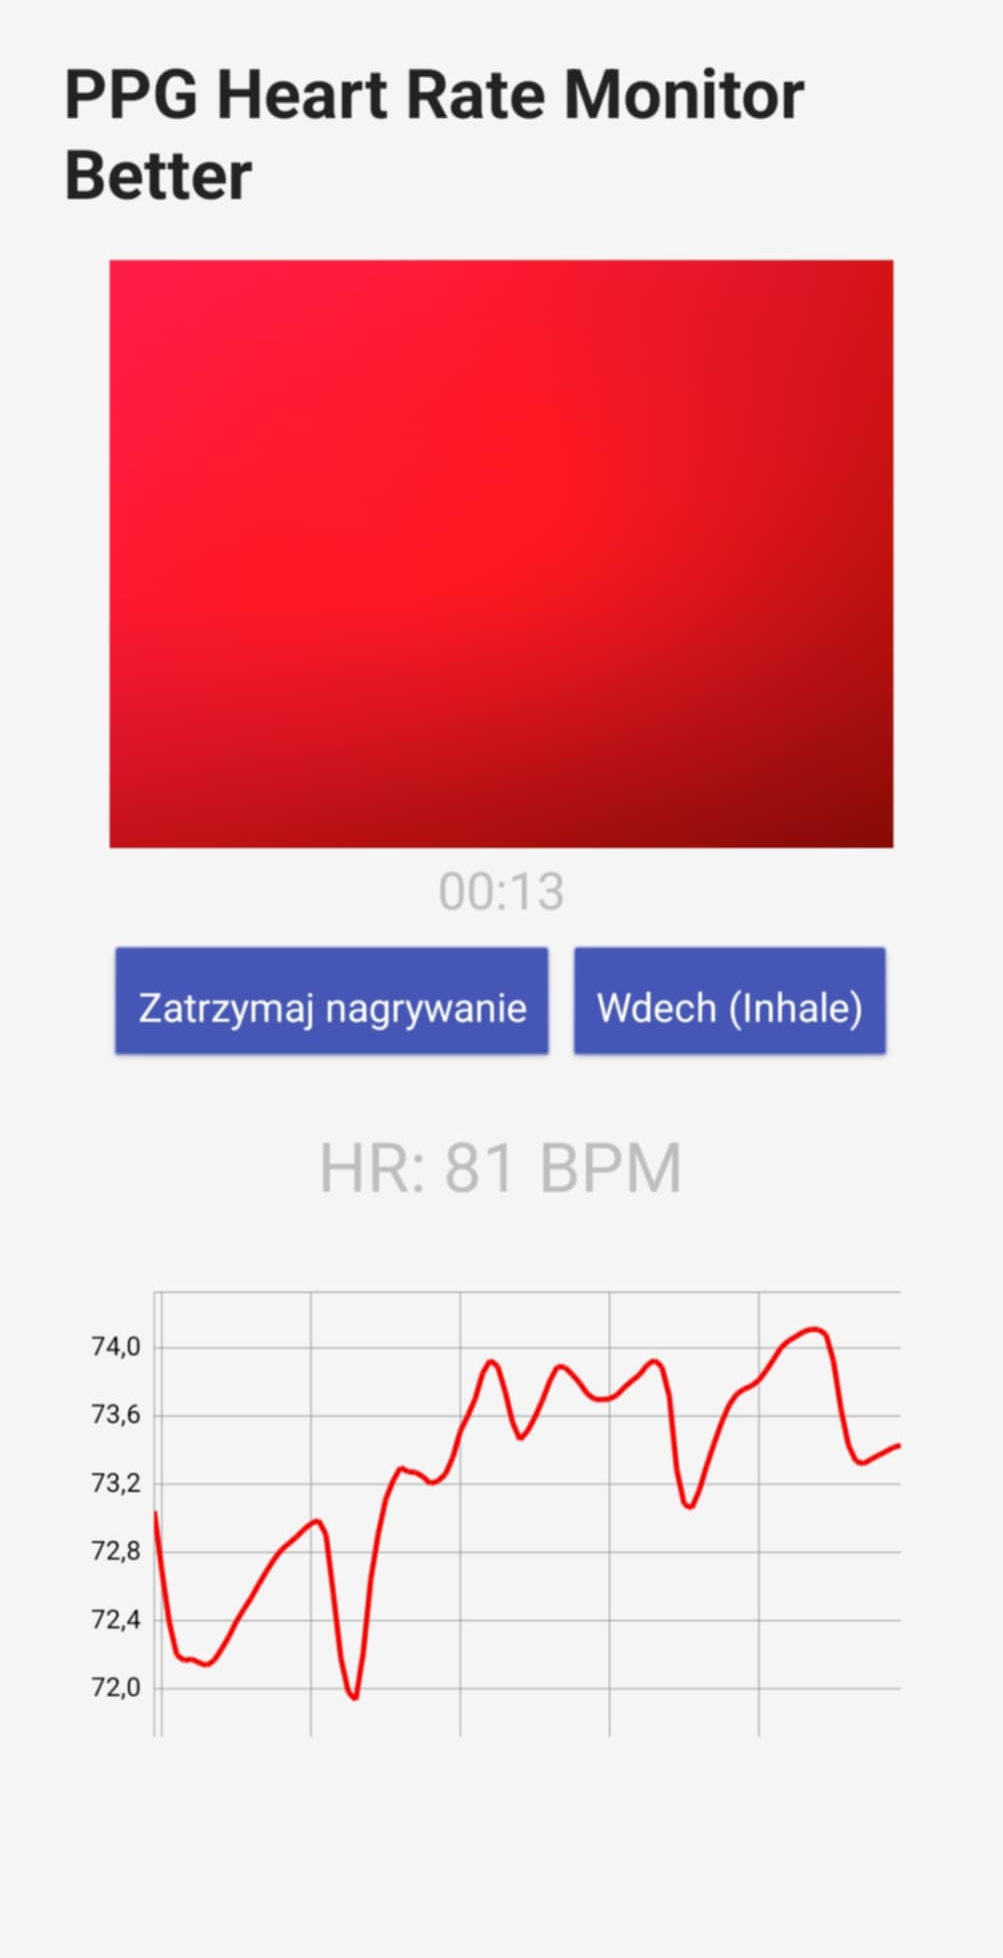
\includegraphics[scale=0.17]{aplikacja.png}
    \caption{Interfejs aplikacji mobilnej}
    \label{fig:aplikacja_mobilna}
\end{figure}

\newpage
Zarejestrowany zapis ulega filtracji dolnoprzepustowej. Detekcja lokalnych maksimów realizowana jest poprzez analizę trzech kolejnych próbek sygnału, środkowy punkt klasyfikowany jest jako szczyt, jeśli jego wartość przewyższa oba sąsiednie. Akceptacja następnego piku wymagana upływu co najmniej 600 ms od poprzedniego wykrycia, ograniczając błędne rozpoznania wynikające z zakłóceń ruchowych. Zidentyfikowane ekstremum jest rejestrowane wraz ze znacznikiem czasu i wykorzystywane do dynamicznego wyznaczania częstości uderzeń serca BPM, zgodnie z równaniem (1) :

\begin{equation}
\text{BPM} = \frac{60}{\Delta t}
\label{eq:bpm}
\end{equation}
gdzie $\Delta t$  - średni odstęp czasowy między kolejnymi pikami sygnału PPG

\paragraph{Proces rejestracji sygnału}
Dane wykorzystane do trenowania i walidacji modelu detekcji szczytów fali zostały pozyskane przy użyciu zaprojektowanej aplikacji. Obrazy przechwytywano w czasie rzeczywistym w formacie YUV 4:2:0 o rozdzielczości 640×480. Z każdej klatki wyodrębniano składową luminancji, na podstawie której obliczano średnią wartość jasności pikseli. Otrzymany odczyt stanowił pojedynczą próbkę surowego sygnału fotopletyzmograficznego.

W celu zgromadzenia odpowiedniego zbioru danych zrealizowano serię pomiarów z udziałem sześciu osób. Każda sesja trwała 10 minut i obejmowała rejestrację sygnału w zróżnicowanych warunkach, uwzględniających drobne ruchy palca wpływające na zmienność przepływu krwi.

\newpage
Transmisję danych pomiędzy smartfonem a komputerem przeprowadzono z wykorzystaniem protokołu WebSocket. Informacje przesyłano w pakietach zawierających pojedyncze punkty pomiarowe wraz z odpowiadającymi im znacznikami czasu. Częstotliwość próbkowania była zgodna z liczbą klatek wideo, wynoszącą około 30 Hz. Odebrane dane buforowano na komputerze i zapisywano w formacie CSV.

\subsection{Filtracja sygnału – filtr Butterwortha}
Filtr Butterwortha opracowano jako rozwiązanie analogowe o maksymalnie płaskiej charakterystyce amplitudowej w paśmie przepustowym, minimalizującej oscylacje i zniekształcenia sygnału. Charakteryzuje się monotonicznym tłumieniem w paśmie zaporowym oraz łagodniejszym zboczem przejściowym niż w strukturach o wyższej selektywności, w tym Czebyszewa i eliptycznych \cite{16}. W implementacji cyfrowej przyjmuje postać układu o nieskończonej odpowiedzi impulsowej IIR, gdzie bieżąca próbka wyjściowa zależy od wartości wejściowych, jak i poprzednich stanów wyjściowych. Podejście to umożliwia realizację filtrów wyższych rzędów przy ograniczonej liczbie współczynników, wykorzystywanych w aplikacjach czasu rzeczywistego \cite{17}.

Do przetwarzania sygnału EKG wykorzystano cyfrowy filtr piątego rzędu o charakterystyce pasmowo-przepustowej, obejmującej zakres częstotliwości od 0,5 Hz do 45 Hz, eliminujący szumy oraz zakłócenia. Dolna granica pasma redukuje powolne zmiany w zapisie wywołane ruchem ciała lub niestabliną pozycją elektrod  \cite{18}. Natomiast górna tłumi zakłócenia sieciowe, elektromagnetyczne oraz mięśniowe  \cite{19}. Filtracja danych została przeprowadzona w oparciu o bibliotekę NeuroKit2.

\begin{figure}[htbp]
    \centering
    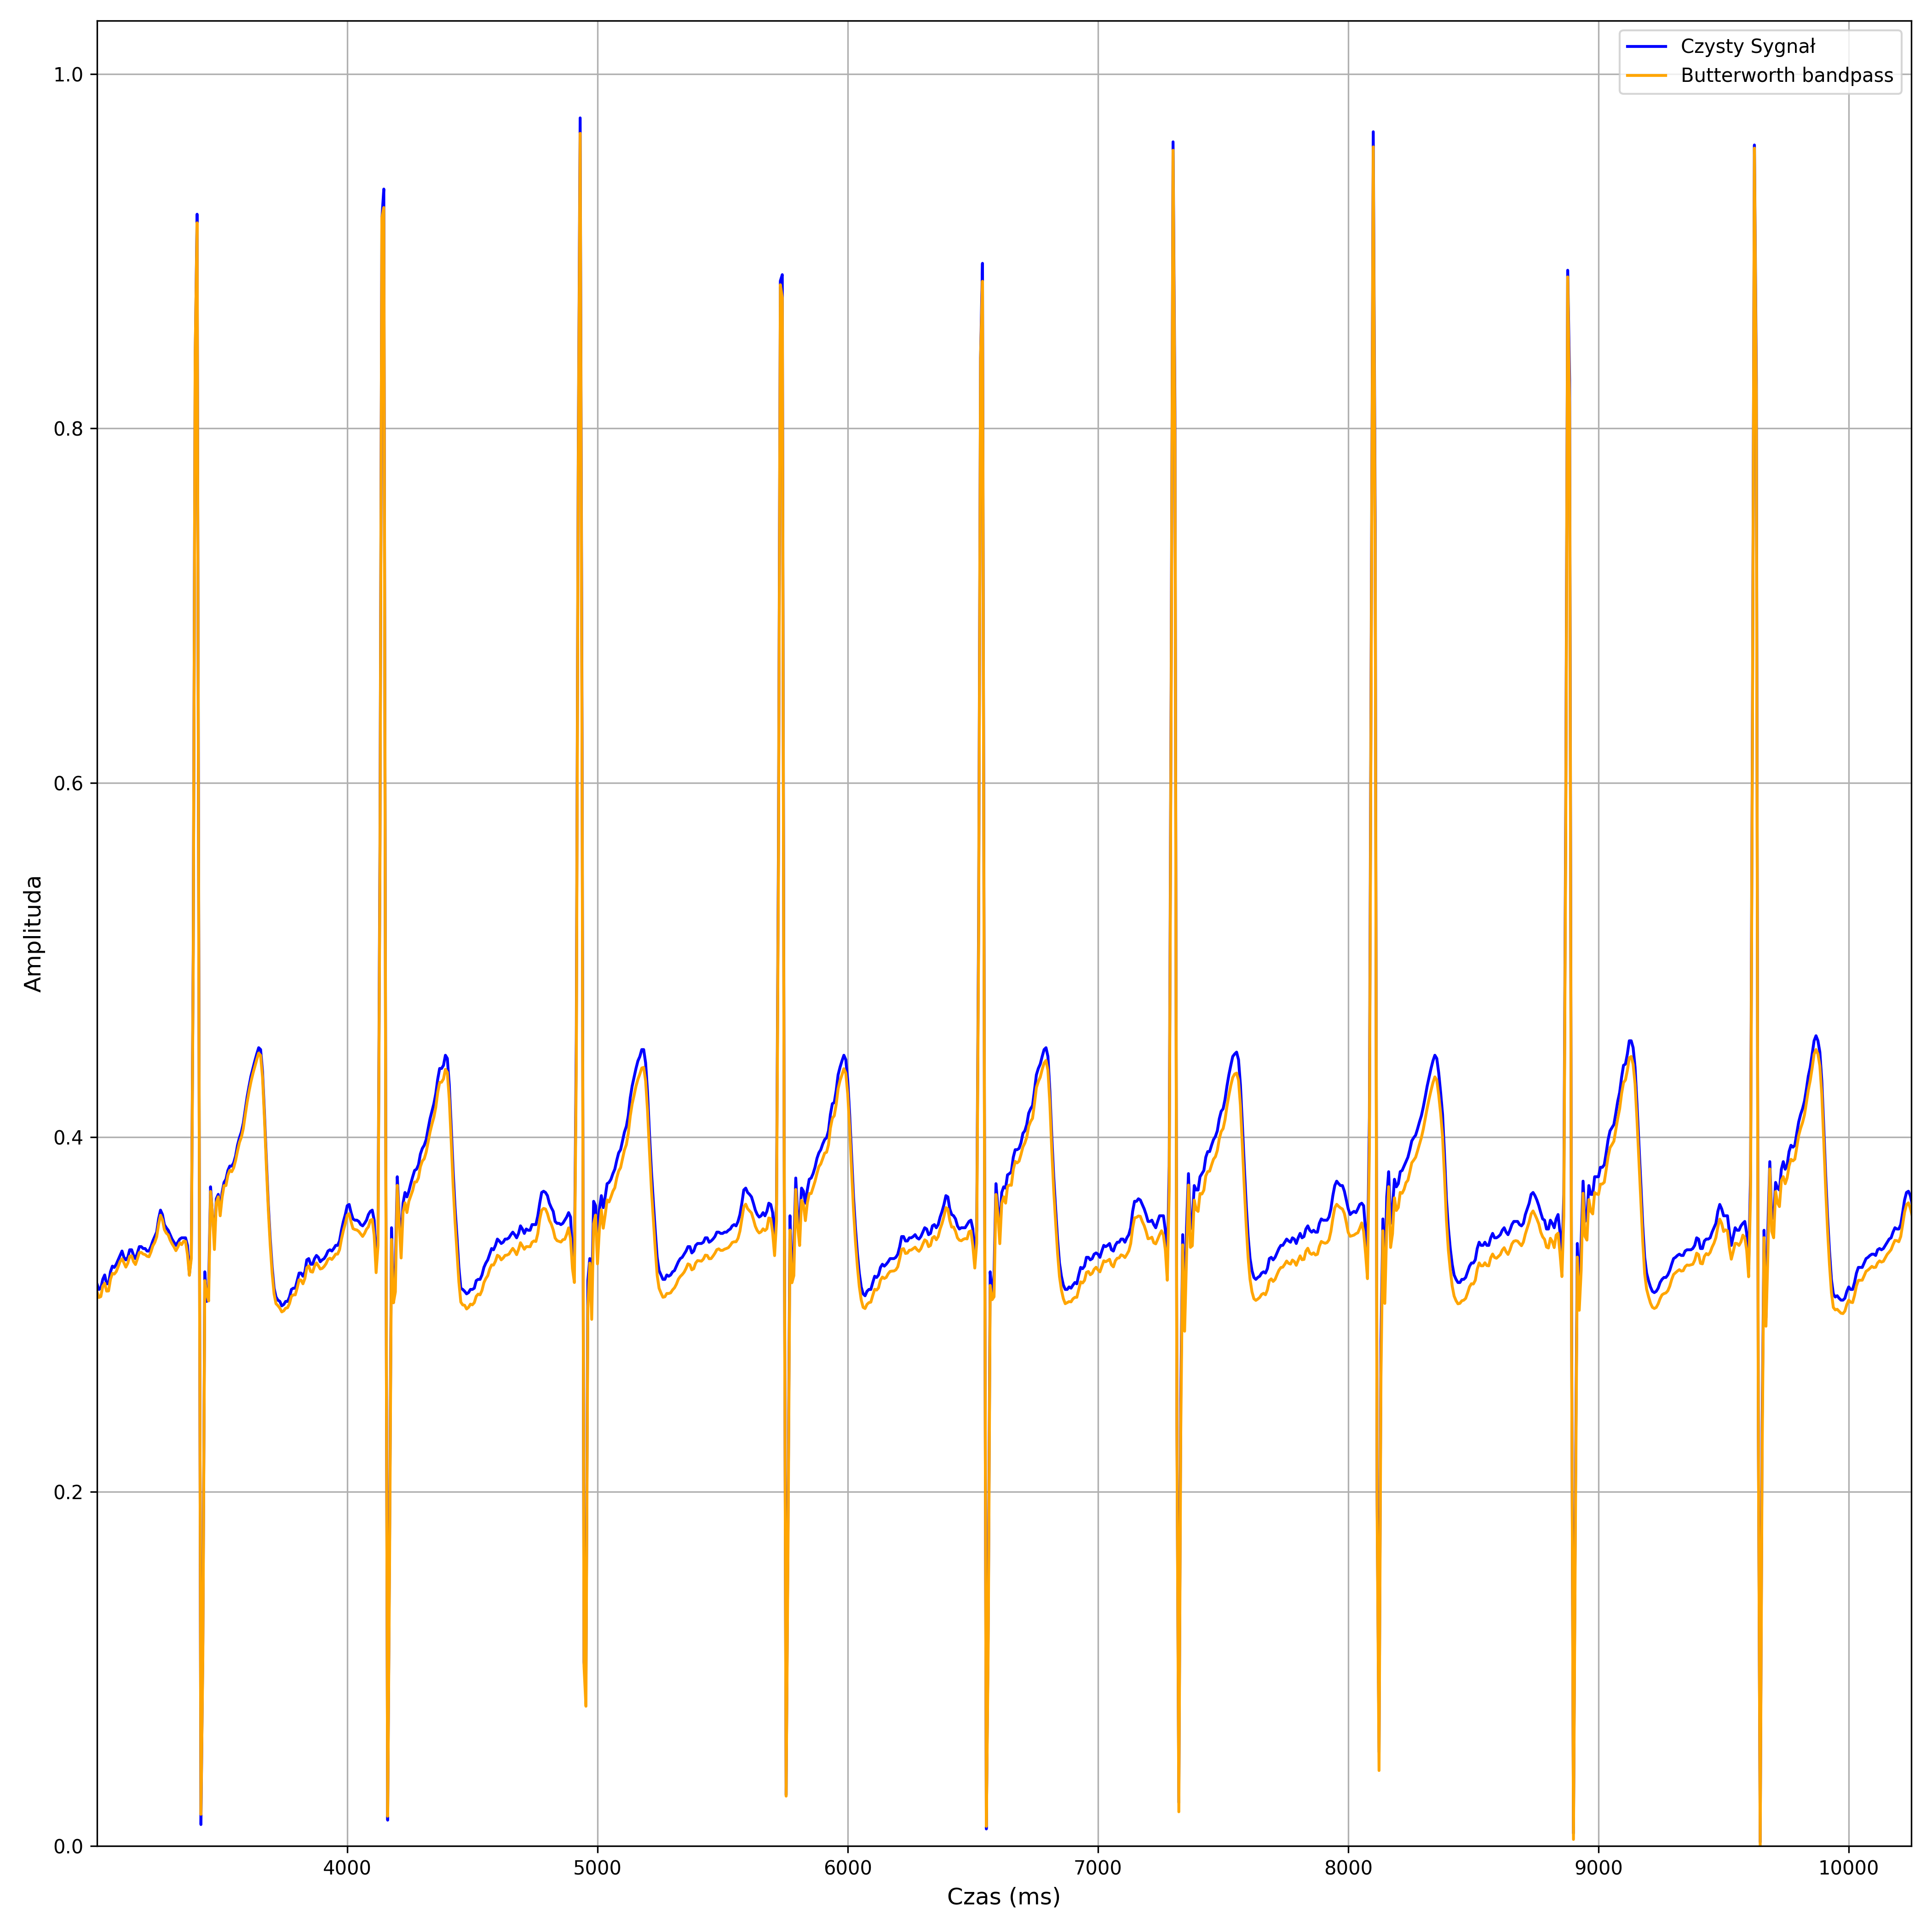
\includegraphics[width=0.76\linewidth]{Filtr_EKG.png} 
    \caption{Porównanie surowego i przefiltrowanego sygnału EKG}
    \label{fig:filtr_ekg}
\end{figure}

\newpage
Dla poprawy jakości sygnału PPG wykorzystano filtr  czwartego rzędu, działający w zakresie 0,5–5 Hz. Dolna granica pasma ogranicza zakłócenia spowodowane ruchem ciała czy niestabilnym kontaktem czujnika ze skórą, natomiast górna tłumi szumy urządzenia pomiarowego i interferencje optyczne  \cite{20}. Filtracja została zrealizowana z wykorzystaniem  modułu SciPy, zapewniając obróbkę przebiegu bez przesunięcia fazowego.

\begin{figure}[htbp]
    \centering
    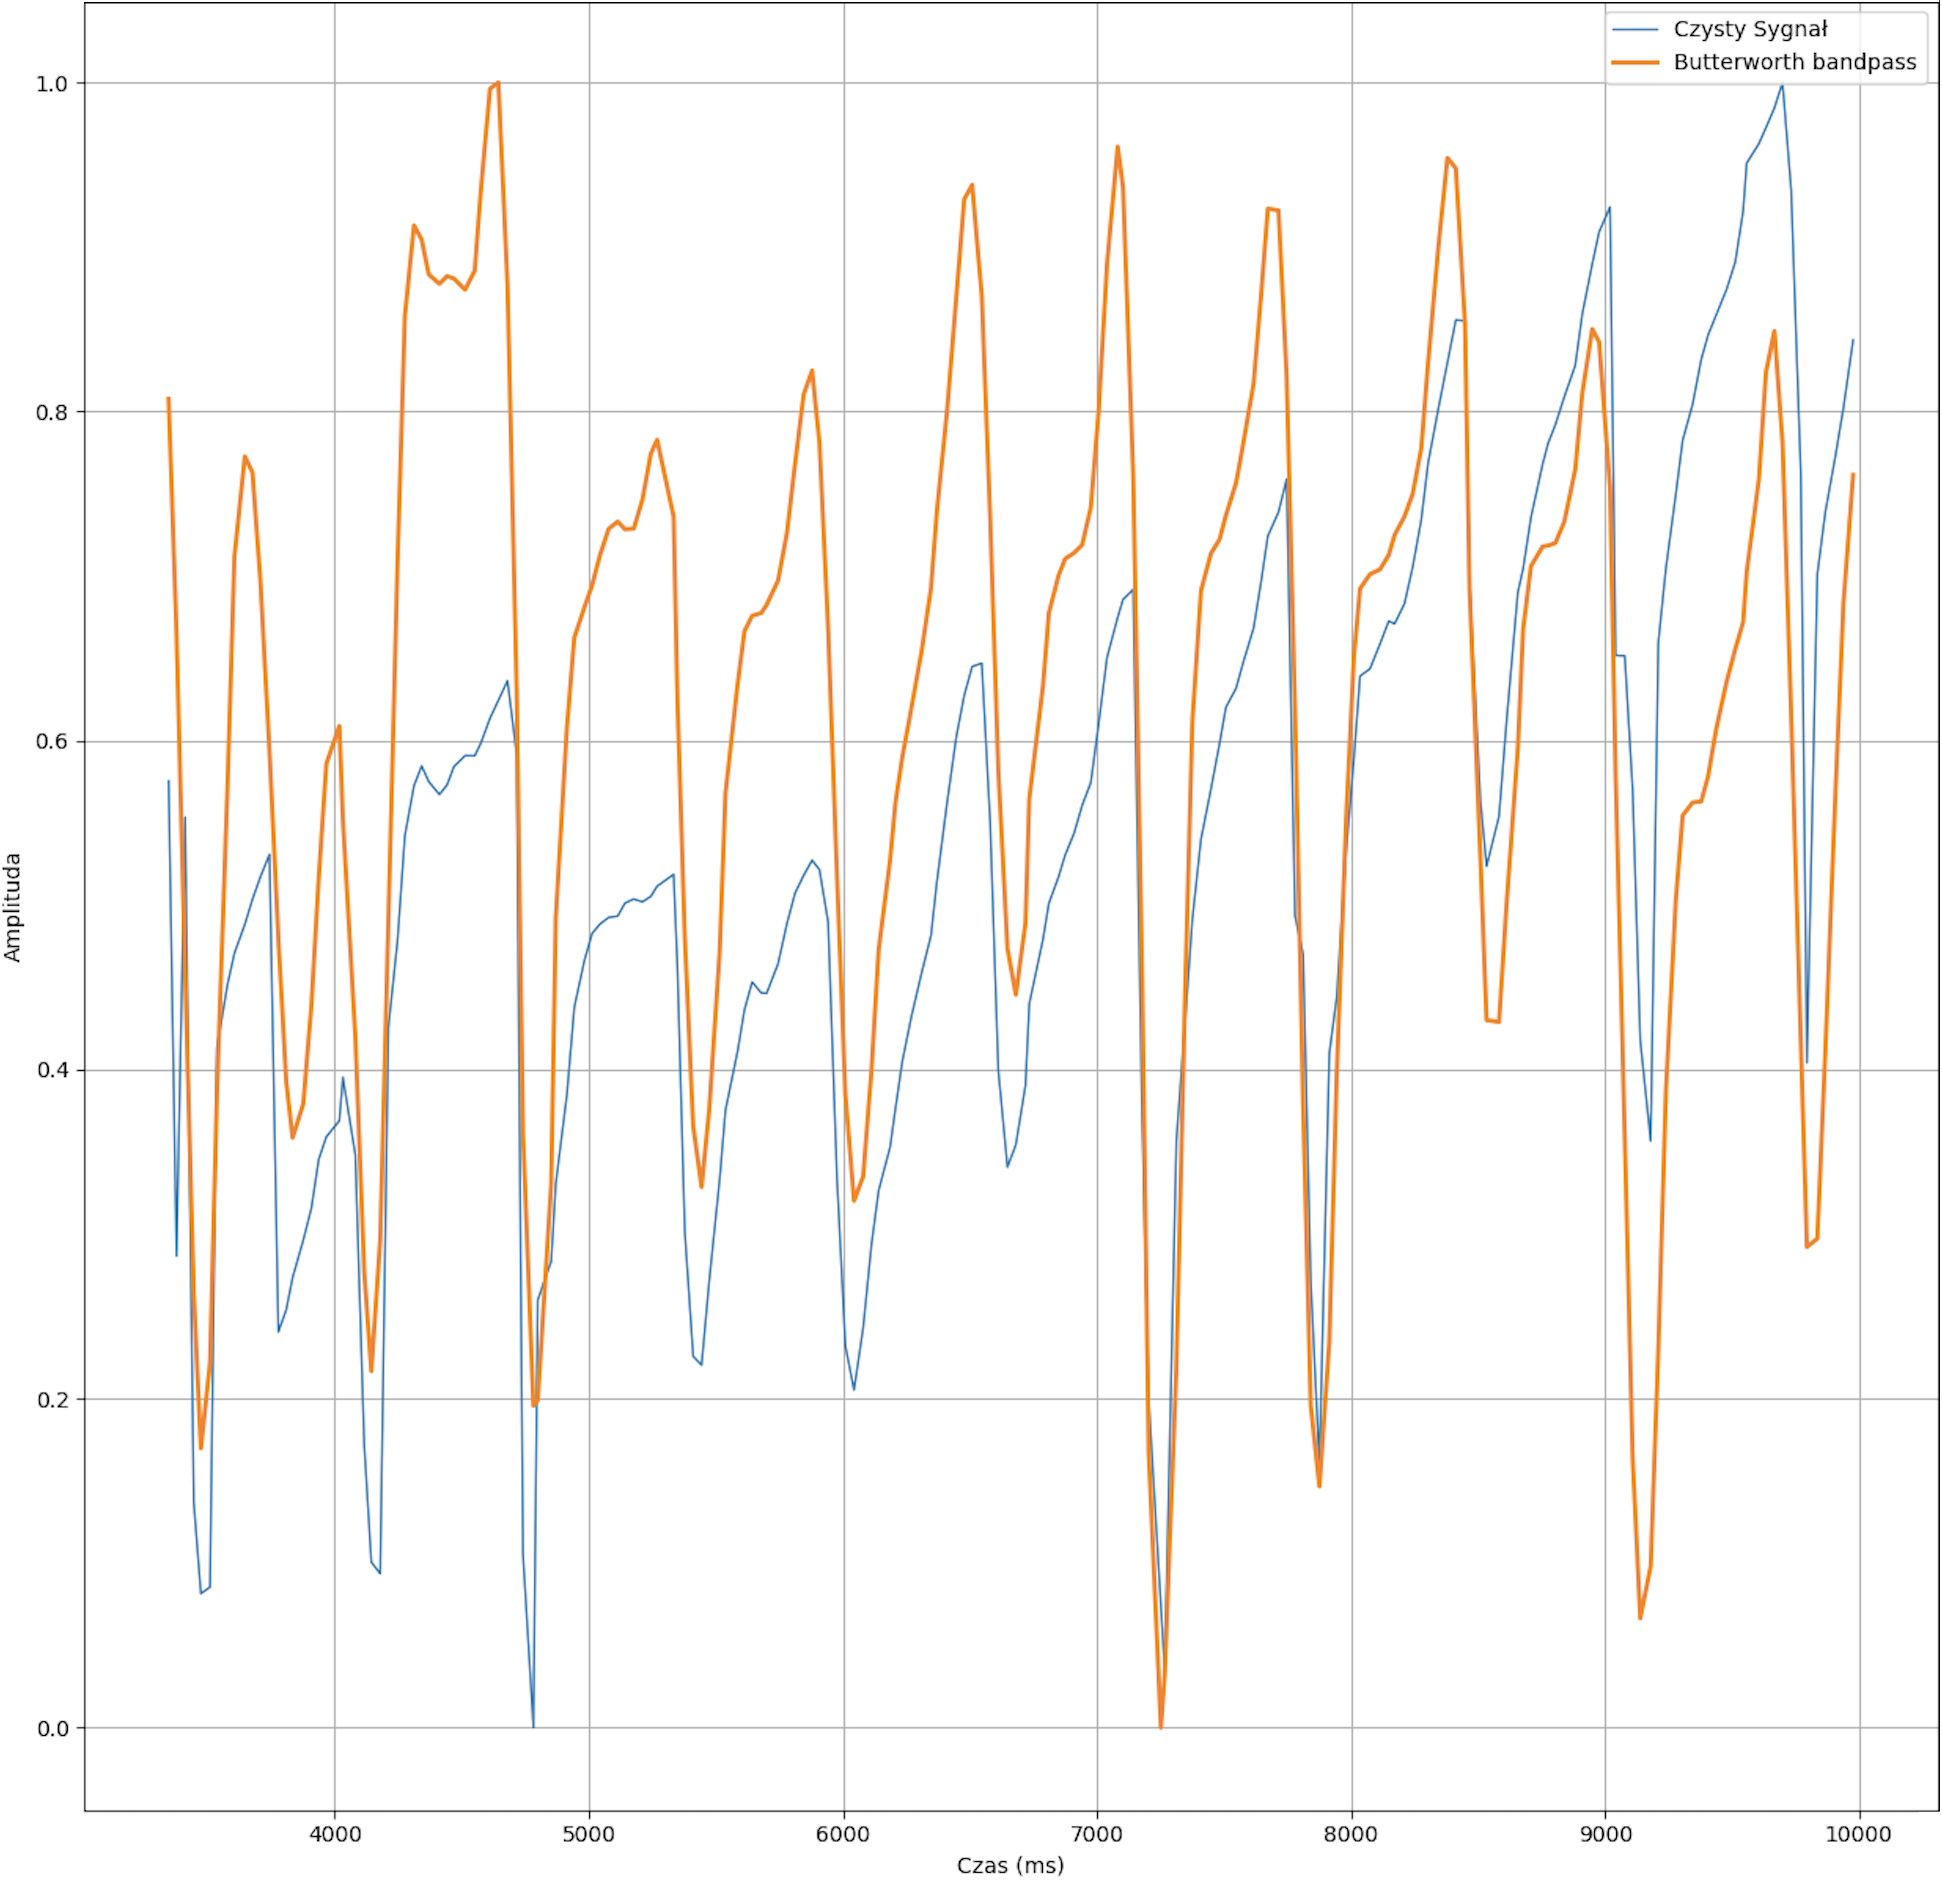
\includegraphics[width=0.76\linewidth]{Filtr_PPG.png} 
    \caption{Porównanie surowego i przefiltrowanego sygnału PPG}
    \label{fig:filtr_ppg}
\end{figure}


\subsection{Modele detekcji}
\subsubsection{Model do wykrywania załamków R}
Opracowano sieć neuronową łączącą warstwy splotowe i rekurencyjne, przeznaczoną do detekcji szczytów R w zapisie EKG. Stanowi ona pierwszy etap w wyznaczaniu interwałów RR i obliczaniu parametrów zmienności rytmu serca. Model przetwarza jednowymiarowe sygnały napięcia elektrycznego podzielone na fragmenty po 256 próbek, stanowiących podstawową jednostkę analizowanego przebiegu.

Część splotowa sieci obejmuje cztery warstwy konwolucyjne 1D, których parametry zestawiono w Tabeli~\ref{tab:conv_layers}. Warstwy te odpowiadają za ekstrakcję cech z sygnału wejściowego, rozszerzając jego reprezentację poprzez zwiększenie liczby kanałów od 16 do 128 za pomocą filtrów o rozmiarach 5 i 3. Dla każdego przekształcenia zastosowano normalizację BatchNorm1d oraz nieliniową funkcję aktywacji LeakyReLU. Redukcja wymiarowości jest realizowana za pomocą operacji MaxPooling1D z jądrem o rozmiarze 2, skracającej długość sekwencji z 256 do 16 próbek wzdłuż osi czasowej oraz zwiększającej odporność modelu na szum i zakłócenia. Wynikowa macierz o wymiarach [128 × 16] stanowi wejście dla jednokierunkowej LSTM. Otrzymany wektor jest spłaszczany i przekazywany do warstwy z 128 neuronami, a następnie do bloku końcowego zawierającego 256 elementów, reprezentujące kolejne próbki sygnału wejściowego.
\newpage
Dane wyjściowe z warstwy LSTM są przetwarzane przez moduły liniowe, odwzorowujące wyekstrahowane cechy w przestrzeń logitów. Każdy element wektora odpowiada prawdopodobieństwu obecności szczytu R w danej próbce, umożliwiając binarną klasyfikację w każdym punkcie czasowym przebiegu. Szczegółowe parametry warstw splotowych uwzględniono w Tabeli~\ref{tab:ecg_layers}.

\begin{table}[h!]
\centering
\caption{Parametry bloków konwolucyjnych sieci}
\label{tab:ecg_layers}
\begin{tabular}{|l|c|c|c|c|c|}
\hline
\textbf{Blok} & \textbf{Wej.} & \textbf{Wyj.} & \textbf{Filtr} & \textbf{Padding} & \textbf{Akt./Norm.} \\
\hline
Conv1D-1 & 1   & 16  & 5 & 2 & LReLU+BN \\
Conv1D-2 & 16  & 32  & 5 & 2 & LReLU+BN \\
Conv1D-3 & 32  & 64  & 3 & 1 & LReLU+BN \\
Conv1D-4 & 64  & 128 & 3 & 1 & LReLU+BN \\
\hline
\end{tabular}
\end{table}

Model wytrenowano w trybie nadzorowanym na podstawie sygnałów pozyskanych z czujnika Polar H10. Rzeczywiste załamki R w przefiltrowanym zapisie EKG wyznaczono algorytmem Pan–Tompkinsa opartym na wieloetapowym przetwarzaniu. Początkową fazą jest pasmowo-przepustowe tłumienie składowych zakłócających o niskiej oraz wysokiej częstotliwości. Różniczkowanie przebiegu uwydatnia strome zbocza zespołu QRS, następnie obliczana jest średnia wartość próbek podniesionych do kwadratu w ruchomym oknie całkującym. Ostateczna detekcja szczytów jest realizowana poprzez progowanie zintegrowanej krzywej oraz analizę lokalnych maksimów \cite{21}.
Każdemu punktowi przypisano etykietę binarną wskazującą obecność lub brak ekstremum, umożliwiając sieci klasyfikację wzorców odpowiadających rzeczywistym pikom R. Proces uczenia przeprowadzono w partiach po 32 elementy z wykorzystaniem funkcji straty BCEWithLogitsLoss. Do optymalizacji zastosowano algorytm Adam przy stałej wartości learning rate wynoszącej 0,0001. Efektywność zaprojektowanej sieci neuronowej oceniono na podstawie wyników uzyskanych na niezależnym zbiorze danych, wykorzystując wytrenowane parametry modelu. Rezultaty klasyfikacji przedstawiono w postaci macierzy konfuzji w Tabeli~\ref{tab:conf_matrix}.

\begin{table}[ht]
\centering
\caption{Macierz konfuzji dla detekcji załamków R}
\label{tab:conf_matrix}
\begin{tabular}{|c|c|c|}
\hline
\textbf{Rzeczywiste / Predykcja} & \textbf{Brak szczytu } & \textbf{Szczyt } \\
\hline
Brak szczytu  & 231170 & 53 \\
Szczyt  & 83 & 2678 \\
\hline
\end{tabular}
\end{table}

Model poprawnie zaklasyfikował 231170 próbek niezawierających piku R oraz 2678 z jego rzeczywistą obecnością. Liczba fałszywie pozytywnych predykcji wyniosła 53, natomiast fałszywie negatywnych -- 83. Wartość miary F1 równa 0,9753 świadczy o wysokiej równowadze pomiędzy precyzją a czułością modelu, co jest kluczowe w automatycznej analizie sygnałów elektrokardiograficznych. Podstawowe metryki oceny jakości modelu przedstawiono w Tabeli~\ref{tab:metrics}.

\newpage
\begin{table}[ht]
\centering
\caption{Parametry detekcji szczytów R}
\label{tab:metrics}
\begin{tabular}{|c|c|p{4.6cm}|}
\hline
\textbf{Metryka} & \textbf{Wartość} & \textbf{Opis} \\
\hline
Skuteczność & 96,99\% & Odsetek poprawnych klasyfikacji obecności lub braku piku R. \\
Błędne detekcje & 0,00\% & Odsetek próbek fałszywie zaklasyfikowanych jako zawierające pik R. \\
Pominięte załamki & 3,01\% & Odsetek próbek z niewykrytym rzeczywistym pikiem R. \\
\hline
\end{tabular}
\end{table}

\subsubsection{Model do wykrywania szczytów fali}
Analogicznie do podejścia zastosowanego w analizie sygnału EKG, opracowano model konwolucyjny identyfikujący lokalne szczyty w przebiegu fotopletyzmograficznym. Stanowi on podstawę do wyznaczania interwałów międzyuderzeniowych IBI, wykorzystywanych przy estymacji wskaźników rytmu serca. Sieć przetwarza dane w postaci wektora zawierającego 50 próbek w pojedynczym kanale, reprezentujących zmiany objętości krwi w naczyniach obwodowych.

Pierwszy element architektury stanowi jednowymiarowa warstwa splotowa z 32 filtrami o szerokości 7 próbek, uzupełniona normalizacją BatchNorm1d oraz funkcją aktywacji GELU, odpowiedzialną za łagodną nieliniowość i poprawę stabilność procesu uczenia. Cztery kolejne bloki resztkowe przetwarzają lokalne wzorce sygnału. Pierwszy moduł zwiększa kanały z 32 do 64, wykorzystując jądro o rozmiarze 9.  Rozszerzenie liczby wymiarów z 64 do 128 realizuje segment przy zastosowaniu okna o długości 5 próbek, natomiast dwa pozostałe utrzymują tę samą głębokość, operując filtrami o wielkości 3 i 7. Transformacje zdefiniowane w początkowym etapie zostały rozszerzone o warstwę Dropout, umożliwiającą redukcję nadmiernego dopasowania. Moduł SE podnosi selektywność modelu, poprawiając precyzję wykrywania lokalnych maksimów przebiegu. Kompresję kanałów z 128 do 64 zapewnia blok konwolucyjny z jądrem o rozmiarze 1, a dwie w pełni połączone operacje liniowe zmniejszają wymiary do 64 i 32, z funkcją aktywacji GELU. Jednowymiarowy wektor wyjściowy podlega transformacji Sigmoid, umożliwiając interpretację wartości jako prawdopodobieństwo lokalnych szczytów w zapisie PPG. Szczegółowe parametry bloków uwzględniono w Tabeli~\ref{tab:ppg_layers}.

\begin{table}[ht]
\centering
\caption{Parametry bloków konwolucyjnych sieci}
\label{tab:ppg_layers}
\begin{tabular}{|l|c|c|c|c|c|}
\hline
\textbf{Blok} & \textbf{Wej.} & \textbf{Wyj.} & \textbf{Filtr} & \textbf{Padding} & \textbf{Akt./Norm.} \\
\hline
Conv1D & 1 & 32 & 7 & 3 & GELU+BN \\
ResidualBlock 1 & 32 & 64 & 9 & 4 & GELU+BN+DO \\
ResidualBlock 2 & 64 & 128 & 5 & 2 & GELU+BN+DO \\
ResidualBlock 3 & 128 & 128 & 3 & 1 & GELU+BN+DO\\
ResidualBlock 4 & 128 & 128 & 7 & 3 & GELU+BN+DO \\
SEBlock & 128 & 128 & – & – & SE scaling \\
Conv1D  & 128 & 64 & 1 & 0 & GELU+BN \\
FC & 128 & 64 & – & – & GELU \\
FC & 64 & 32 & – & – & GELU \\
Output & 32 & 1 & – & – & Sigmoid \\
\hline
\end{tabular}
\end{table}

\newpage
Proces uczenia nadzorowanego dla danych PPG przeprowadzono na segmentach sygnału pochodzących z urządzenia mobilnego, poddanych wstępnej filtracji i normalizacji do zakresu [-1, 1]. W każdym wycinku przypisano wektor etykiet binarnych określający obecność lub brak piku, oparty na identyfikacji lokalnych szczytów przewyższających sąsiednie wartości, umożliwiając klasyfikację wzorców w obrębie okna. Sieć trenowano na 50-punktowych fragmentach przebiegu, w partiach po 32 segmenty, wykorzystując funkcję straty BCELoss oraz optymalizator Adam ze stałym współczynnikiem uczenia równym 0,001. Skuteczność zaprojektowanego modelu oceniono na podstawie wyników uzyskanych na niezależnym zbiorze danych, przy zastosowaniu parametrów wyznaczonych podczas dopasowania. Wyniki klasyfikacji przedstawiono w formie macierzy konfuzji w Tabeli~\ref{tab:conf_matrix_ppg}.

\begin{table}[ht]
\centering
\caption{Macierz konfuzji dla detekcji pików fali}
\label{tab:conf_matrix_ppg}
\begin{tabular}{|c|c|c|}
\hline
\textbf{Rzeczywiste / Predykcja} & \textbf{Brak szczytu } & \textbf{Szczyt} \\
\hline
Brak szczytu  & 9609 & 9 \\

Szczyt  & 7 & 375 \\
\hline
\end{tabular}
\end{table}

Dla sygnałów fotopletyzmograficznych sieć poprawnie rozpoznała 9609 próbek bez obecności fali oraz 375 z jej wystąpieniem. Niepoprawne predykcje odnotowano w 9 przypadkach fałszywie dodatnich oraz 7  fałszywie ujemnych. Otrzymana wartość miary F1, wynosząca 0,9774, jest zbliżona do wyników uzyskanych dla modelu EKG, potwierdzając wiarygodność zastosowanego rozwiązania w analizie obu typów sygnałów.
Podstawowe metryki oceny jakości architektury przedstawiono w Tabeli~\ref{tab:metrics_ppg}.

\begin{table}[ht]
\centering
\caption{Parametry detekcji szczytów fali}
\label{tab:metrics_ppg}
\begin{tabular}{|c|c|p{4.6cm}|}
\hline
\textbf{Metryka} & \textbf{Wartość} & \textbf{Opis} \\
\hline
Skuteczność & 98,17\% & Odsetek poprawnych klasyfikacji obecności lub braku piku fali. \\
Błędne detekcje & 0,52\% & Odsetek próbek fałszywie zaklasyfikowanych jako zawierające pik fali. \\
Pominięte załamki & 1,83\% & Odsetek próbek z niewykrytym rzeczywistym pikiem fali. \\
\hline
\end{tabular}
\end{table}

\newpage
\section{Ewaluacja maksimów i analiza czasowa sygnałów biomedycznych}
\subsection{Weryfikacja skuteczności detekcji pików R}
Skuteczność architektury opartej na sieci splotowej w wykrywaniu pików R w zapisie elektrokardiograficznym oceniono względem klasycznego algorytmu Pan–Tompkinsa oraz szczytów referencyjnych uzyskanych w ramach biblioteki NeuroKit, pełniącej rolę złotego standardu. Sygnał próbkowano z częstotliwością 130 Hz i przetwarzano w niepokrywających się segmentach obejmujących 256 próbek. 

Łączna wartość wykrytych maksimów wyniosła 54 dla modelu, 56 metodą Pan-Tompkinsa oraz 56 w danych wzorcowych. Wyniki przedstawiono w Tabeli~\ref{tab:peak_comparison}, zawierającej liczbę prawdziwych trafień TP, fałszywych alarmów FP, pominiętych szczytów FN, wraz z obliczonymi wskaźnikami precyzji, czułości i F1, przy tolerancji odpowiadającej 1–2 punktom przebiegu.

\begin{table}[ht]
\caption{Ocena technik wyznaczania ekstremów}
\label{tab:peak_comparison}
\centering
\begin{tabular}{|p{3.08cm}|c|c|c|c|c|c|}
\hline
\textbf{Metoda} & \textbf{TP} & \textbf{FP} & \textbf{FN} & \textbf{Prec.} & \textbf{Czuł.} & \textbf{F1} \\
\hline
AI vs Pan-Tompkins & 54 & 0 & 2 & 1.000 & 0.964 & 0.982 \\
AI vs NeuroKit & 53 & 1 & 3 & 0.981 & 0.946 & 0.964 \\
Pan-Tompkins vs NeuroKit & 55 & 1 & 1 & 0.982 & 0.982 & 0.982 \\
\hline
\end{tabular}
\end{table}

\begin{figure}[htbp]
    \centering
    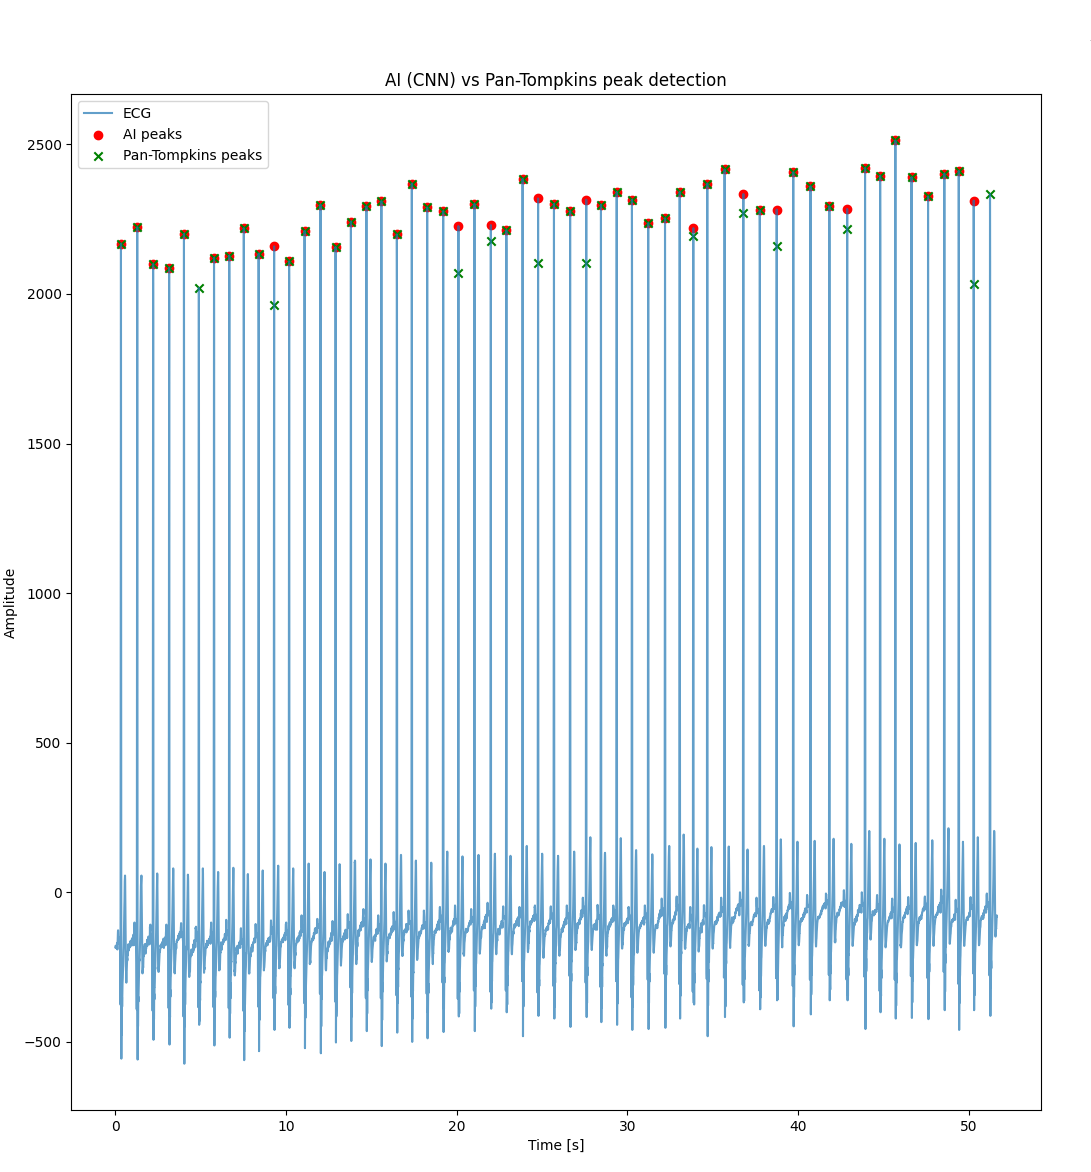
\includegraphics[scale=0.2]{ai_pan-tompkins.png}
    \caption{Porównanie detekcji pików R przez sieć splotową z algorytmem Pan-Tompkinsa}
    \label{fig:ai_pan-tompkins}
\end{figure}

\begin{figure}[htbp]
    \centering
    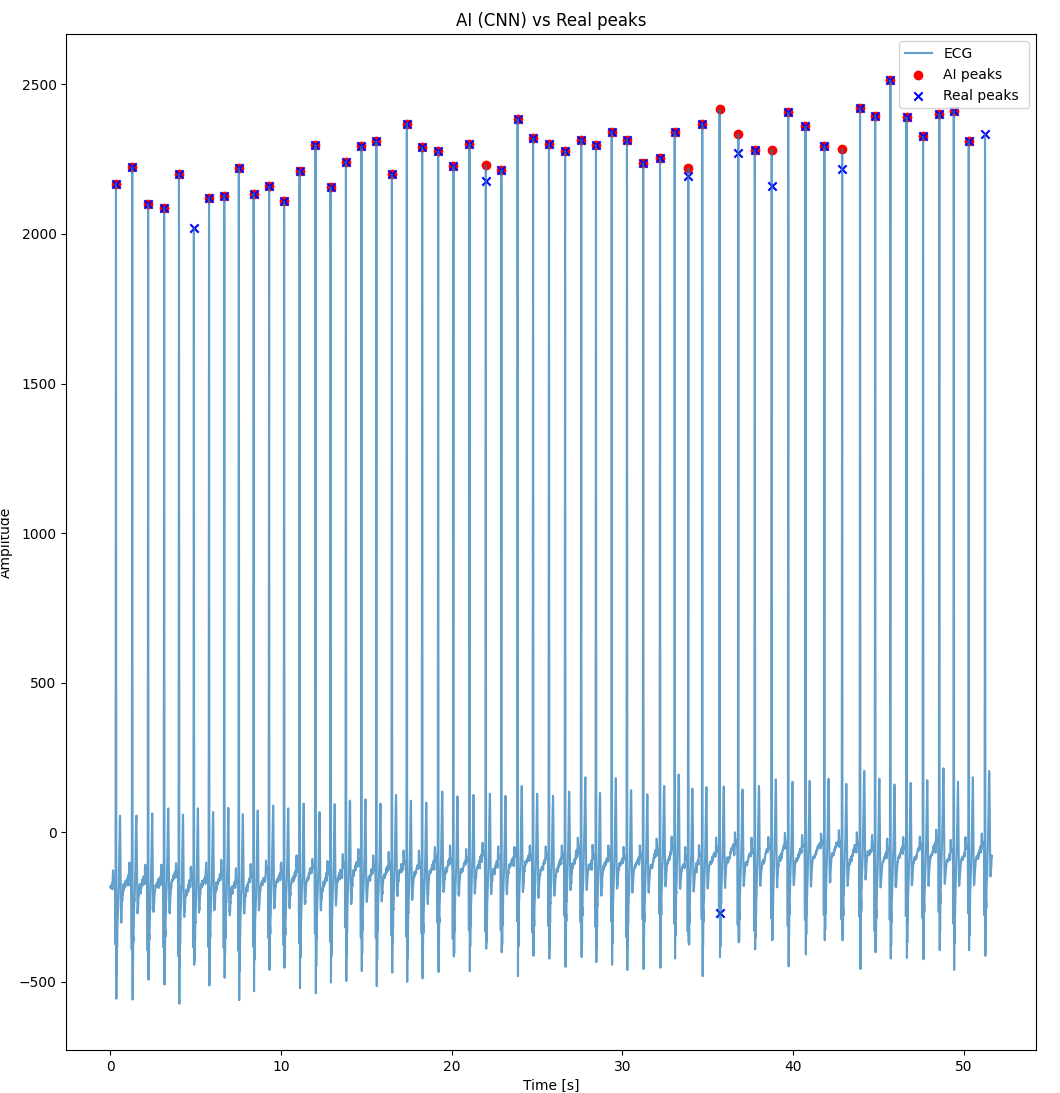
\includegraphics[scale=0.2]{ai_real_peaks.png}
    \caption{Porównanie detekcji pików R przez sieć splotową z szczytami referencyjnymi}
    \label{fig:ai_real_peaks}
\end{figure}


\newpage
Skuteczność sieci w wykrywaniu pików R jest porównywalna z klasycznym algorytmem Pan-Tompkinsa i charakteryzuje się wysoką zgodnością z wartościami referencyjnymi. Rozbieżności wynikające z pominiętych lub przesuniętych ekstremów można zredukować poprzez optymalizację wstępnej obróbki sygnału lub dalsze trenowanie modelu. Obecne systemy uczenia maszynowego wykazują zdolność do osiągania niemal najwyższej klasy skuteczności w automatycznym wykrywaniu lokalnych szczytów zapisu elektrokardiograficznego.

\subsection{Weryfikacja skuteczności detekcji pików fali}
Identyfikacje szczytów przebiegu fotopletyzmograficznego przeprowadzono na podstawie wyników sieci konwolucyjnej oraz sygnału referencyjnego uzyskanego metodą filtracji pasmowo-przepustowej i lokalnego wyszukiwania maksimów. Dane podzielono na segmenty o długości 100 próbek i znormalizowano do zakresu [−1,1]. W trybie okienkowym predykcje modelu przekształcono w indeksy punktów odpowiadających potencjalnym pikom fali.

Algorytm uczenia maszynowego wykrył 76 szczytów, natomiast zestaw wzorcowy obejmował 72. Skuteczność detekcji przebiegła w przedziale tolerancji 264 ms, odpowiadającym 8 jednostkom czasowym przy częstotliwości próbkowania 30 Hz, z zastosowaniem parametrów prawdziwych trafień TP, fałszywych alarmów FP oraz pominiętych pików FN. Model uzyskał 61 TP, 15 FP oraz 11 FN, przekładając się na precyzję 0,803, czułość 0,847 oraz miarę F1 równą 0,824.

\begin{figure}[htbp]
    \centering
    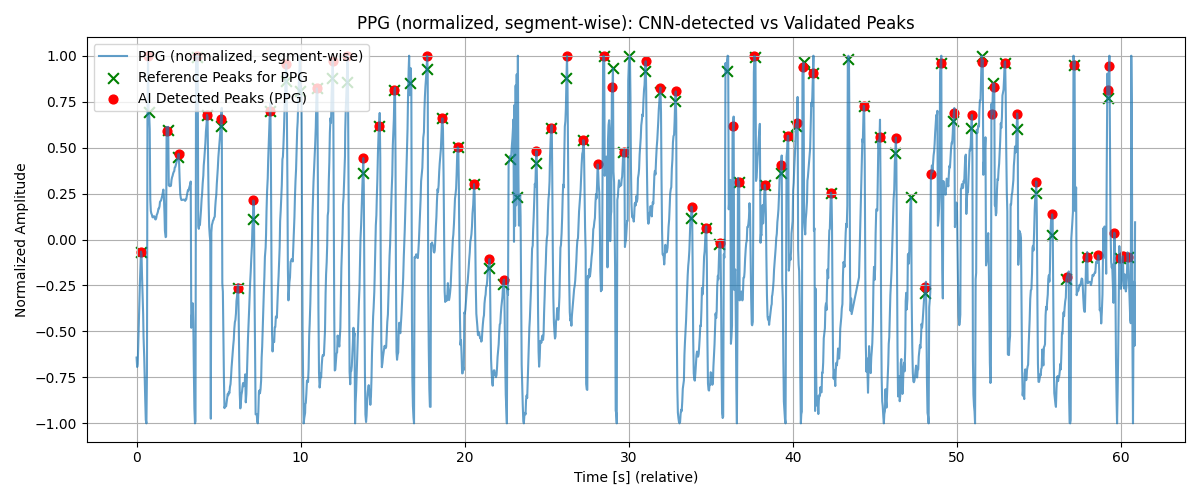
\includegraphics[scale=0.28]{ppg_ai_vs_real.png}
    \caption{Porównanie detekcji pików fali przez sieć splotową z szczytami referencyjnymi}
    \label{fig:ppg_ai_real_peaks}
\end{figure}

\newpage
Wyniki wskazują na wysoką zgodność architektury z referencyjnymi maksimami przebiegu fotopletyzmograficznego, przy niewielkiej liczbie fałszywego wykrywania spowodowanego zakłóceniami i ograniczeniami analizy krótkich segmentów. Uzyskane rezultaty sugerują praktyczną użyteczność sieci w cyfrowym przetwarzaniu sygnałów biomedycznych.


\subsection{Estymacja PTT ze zsynchronizowanych sygnałów}
Podczas rejestracji sygnałów EKG i PPG wykorzystywane są różne schematy zapisu znaczników czasowych. W elektrokardiogramie punkty wystąpienia załamków R początkowo określane są względem chwili rozpoczęcia akwizycji i zapisywane w sekundach jako czas względny. Podczas przetwarzania danych wartości te są przekształcane do formatu absolutnego UNIX, umożliwiając porównanie z przebiegiem PPG. W fotopletyzmografii detekcja szczytów fali rejestrowana jest bezpośrednio w czasie systemowym.

Dla ujednolicenia układu czasowego przekształca się dane EKG z czasu względnego na znaczniki UNIX, zgodnie z równaniem (2):
\begin{equation}
t_{\mathrm{UNIX}} = t_{\mathrm{rel}} + t_{0},
\end{equation}
gdzie $t_{\mathrm{UNIX}}$ - czas w formacie UNIX, $t_{\mathrm{rel}}$ – czas względny, a $t_{0}$ – początek akwizycji.

Przebiegi zostały przedstawione w jednej osi czasu, umożliwiając ich automatyczną synchronizację. Dopasowanie par szczytów realizowano poprzez przypisanie do każdego załamka R w zapisie elektrokardiograficznym najbliższego w kolejności wystąpień ekstremum w sygnale fotopletyzmograficznym. Nie każdy zarejestrowany pik w EKG posiada odpowiadający punkt w PPG, wynikający z zakłóceń ruchowych lub utraty próbek. Różnice czasowe między dopasowanymi maksimami definiowane są jako interwał propagacji tętna PTT, wyznaczany zgodnie z równaniem (3):
\begin{equation}
PTT = t_{\mathrm{PPG}} - t_{\mathrm{ECG}},
\end{equation}
gdzie $t_{\mathrm{PPG}}$, $t_{\mathrm{ECG}}$ - momenty detekcji szczytów w przebiegu PPG i EKG. 

\newpage
\begin{figure}[htbp]
    \centering
    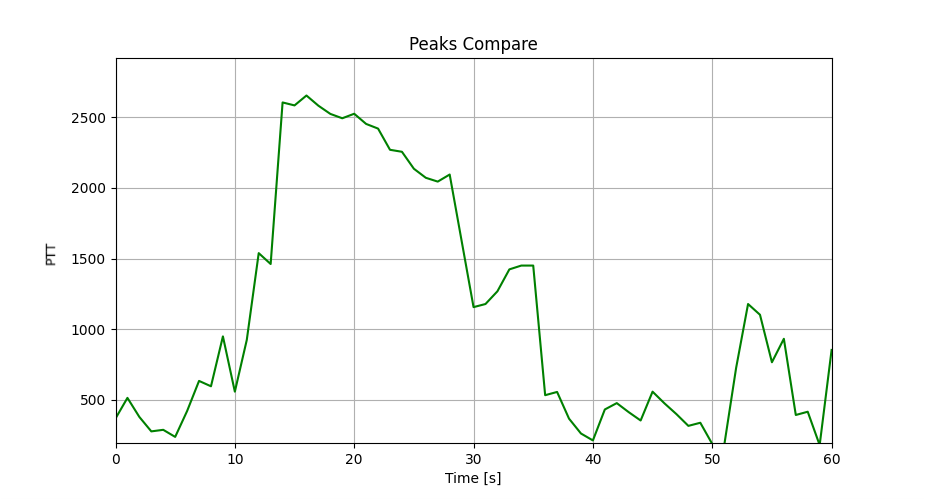
\includegraphics[width=1.0\linewidth]{Peaks_compare.png}
   \caption{Chwilowe różnice czasowe między szczytami EKG i PPG}
    \label{fig:PTT}
\end{figure}

Z wektora wartości wyznacza się statystyki opisowe, obejmujące średnią, określającą przeciętny czas przejścia fali tętna, oraz odchylenie standardowe, wyrażające jego zmienność.

\subsection{Wskaźniki HRV}
Odstępy między kolejnymi uderzeniami serca analizowano niezależnie w obu sygnałach. W elektrokardiografii wykorzystano czas względny, wynikający z okienkowego trybu przetwarzania próbek, natomiast w fotopletyzmografii zastosowano znaczniki systemowe, zapewniając spójność z rejestrowanym przebiegiem oraz umożliwiając synchronizację z innymi źródłami danych. Dla zapisu EKG określono interwały RR, odpowiadające odległościom między załamkami R, a w PPG odstępy międzyuderzeniowe IBI. Na podstawie tych wartości wyznaczono standardowe parametry HRV, przedstawione w formie RR. Analogiczne obliczenia przeprowadzono dla IBI.

\noindent\textit{1) Średnia długość interwału:} 
Średnia arytmetyczna odstępów RR, wyrażona wzorem (4):
\begin{equation}
    Mean = \frac{1}{N} \sum_{i=1}^{N} RR_i
\end{equation}
gdzie $RR_i$ -- $i$-ty odstęp RR, a $N$ – liczba analizowanych odstępów.

\noindent\textit{2) Odchylenie standardowe odstępów NN:} 
Wielkość całkowitej zmienności rytmu serca, obliczana na podstawie wszystkich interwałów RR, wyrażona wzorem (5):
\begin{equation}
    SDNN = \sqrt{\frac{1}{N-1} \sum_{i=1}^{N} (RR_i - Mean)^2}
\end{equation}
gdzie $Mean$ – średnia długość interwału, $RR_i$ – $i$-ty odstęp RR, a $N$ – liczba analizowanych odstępów. \textbf{}

\noindent\textit{3) Pierwiastek kwadratowy z uśrednionych kwadratów różnic kolejnych odstępów NN:} 
Miara stosowana w ocenie krótkoterminowych wahań rytmu serca, wyrażona wzorem (6):
\begin{equation}
    RMSSD = \sqrt{\frac{1}{N-1} \sum_{i=1}^{N-1} (RR_{i+1} - RR_i)^2}
\end{equation}
gdzie $RR_i$ -- $i$-ty odstęp RR, a $N$ – liczba analizowanych odstępów.

Do obliczeń w czasie rzeczywistym wykorzystano dynamiczne okno o długości 60 s. Oznaczenia pików oraz odpowiadające im odstępy są aktualizowane w trybie online, natomiast próbki spoza okna są usuwane. Parametry SDNN, RMSSD oraz średnie interwały między uderzeniami serca przedstawiono w postaci wykresów.

\begin{figure}[h]
    \centering
    \begin{subfigure}{0.47\textwidth}
        \centering
        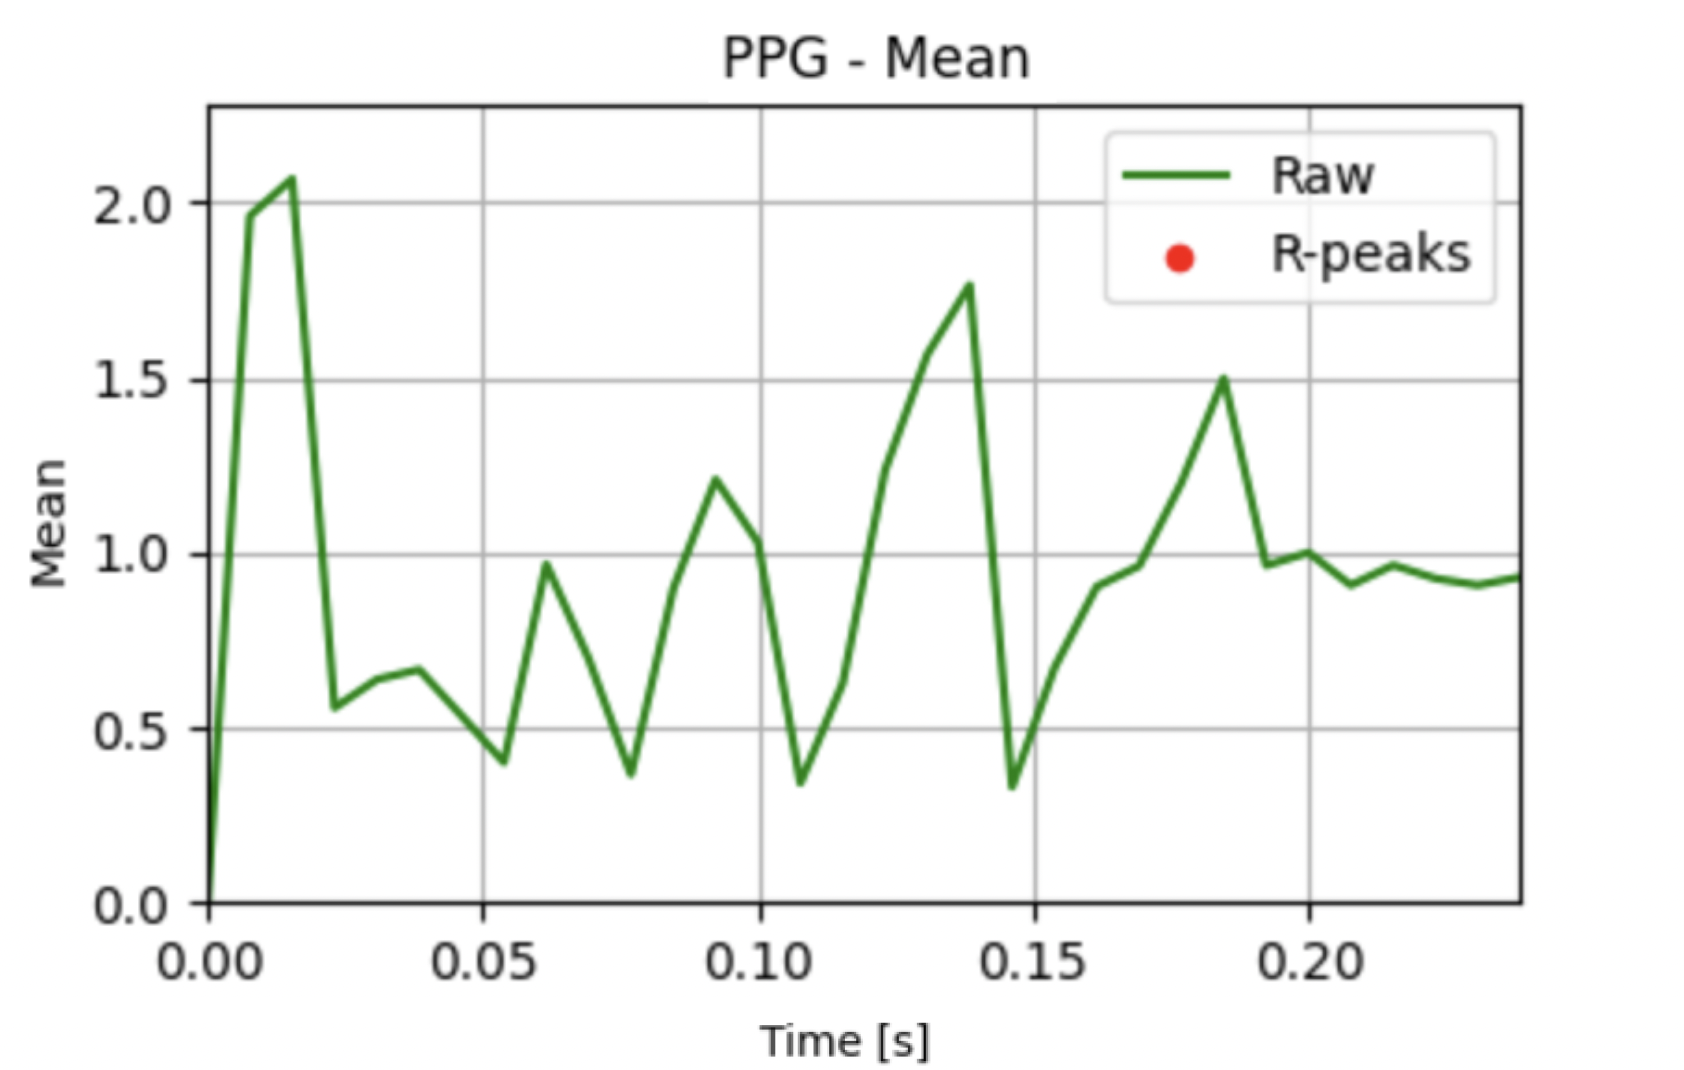
\includegraphics[width=\linewidth]{Mean.png}
        \caption{Średnia długość interwału}
    \end{subfigure}
    
   \vspace{0.3cm} 
    \begin{subfigure}{0.47\textwidth}
        \centering
        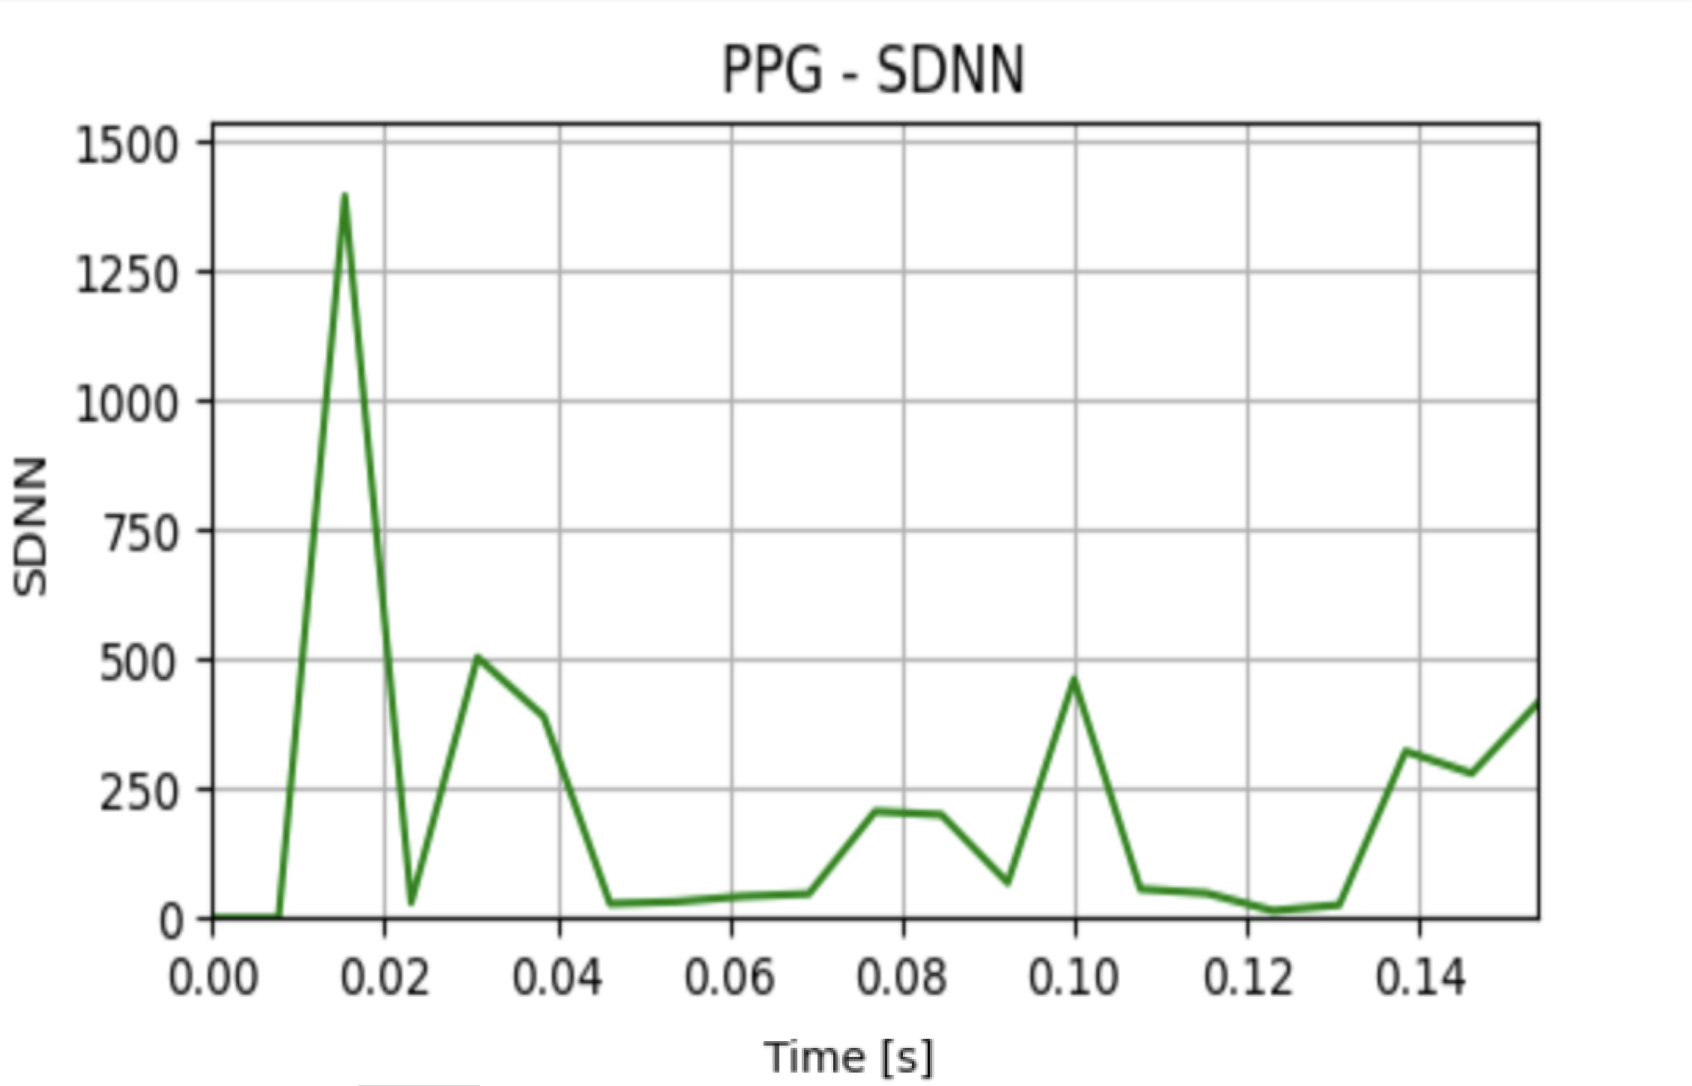
\includegraphics[width=\linewidth]{SDNN.png}
        \caption{Odchylenie standardowe odstępów NN}
    \end{subfigure}
    
    \vspace{0.3cm}  
    \begin{subfigure}{0.47\textwidth}
        \centering
        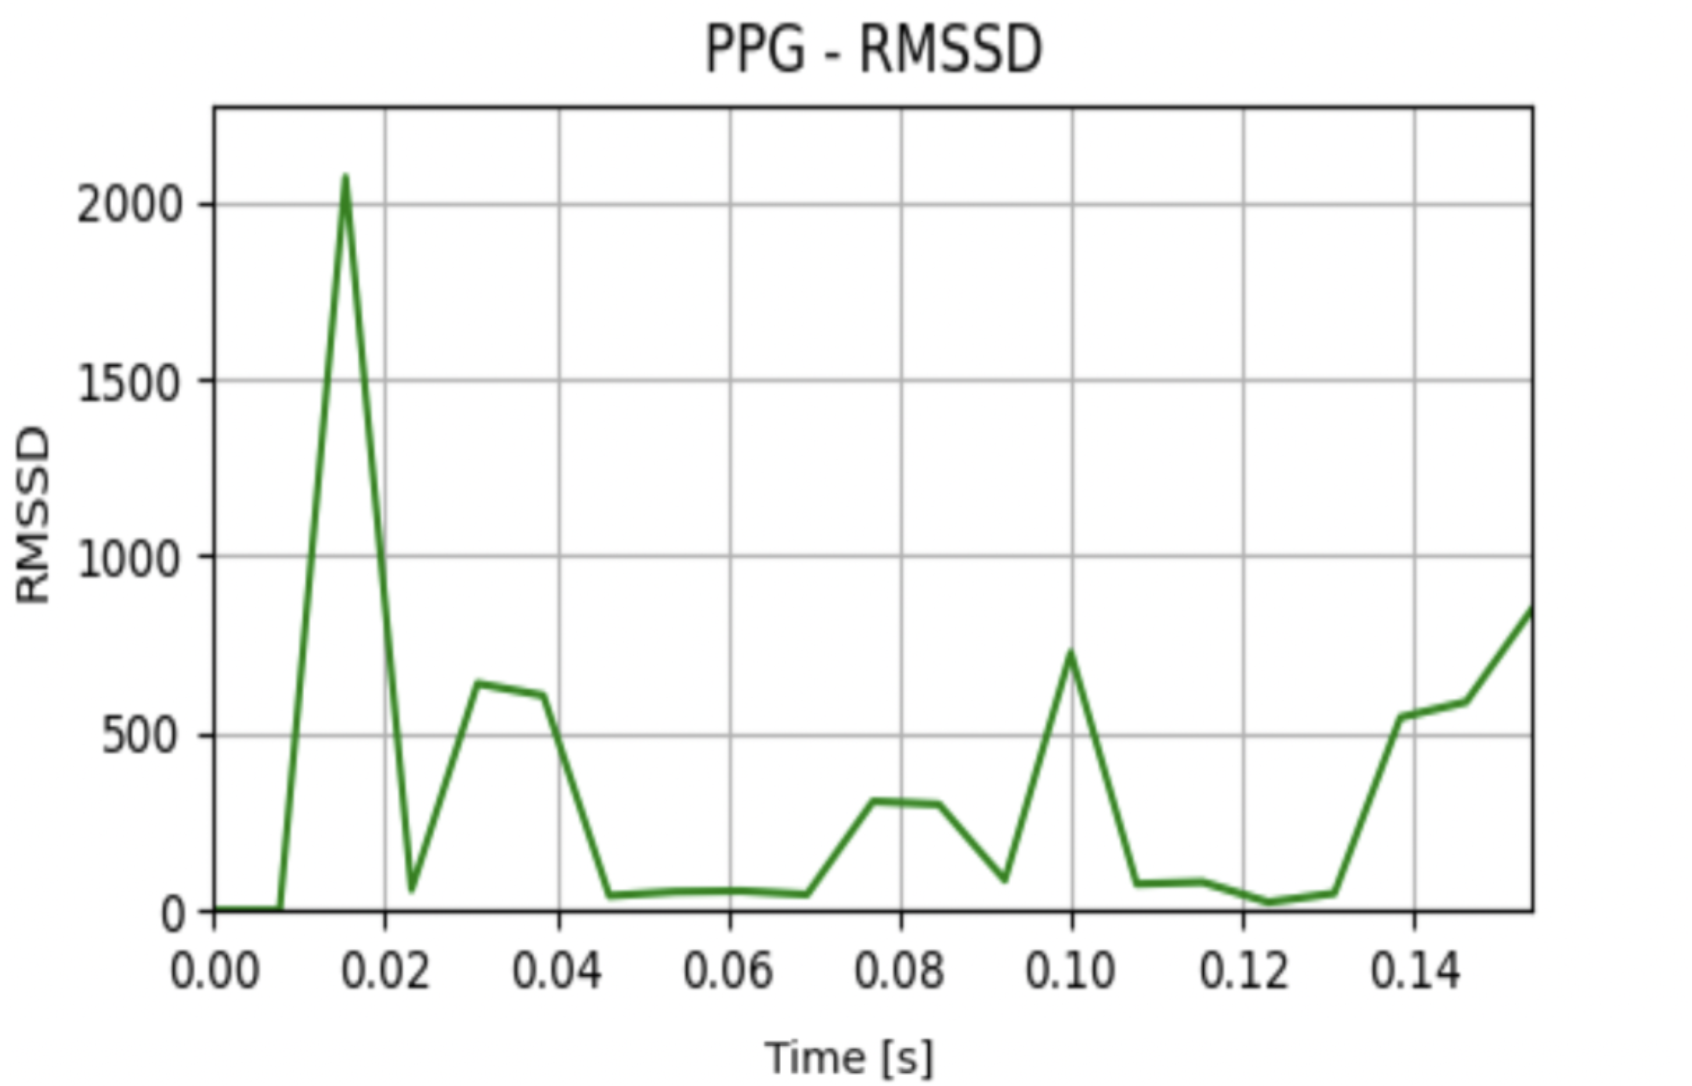
\includegraphics[width=\linewidth]{RMSSD.png}
        \caption{Pierwiastek kwadratowy średniej z kwadratów różnic  odstępów NN}
    \end{subfigure}  
    \caption{Przykładowe przebiegi wskaźników HRV wyznaczone dla PPG}
\end{figure}

\newpage
\section{Zakończenie}
Ewaluacja wykazała, że zastosowane architektury splotowe i rekurencyjne zapewniają wysoką zgodność z klasycznymi metodami oraz danymi wzorcowymi, przy jednoczesnym ograniczeniu liczby fałszywych detekcji. Uzyskane wartości miary F1 potwierdzają skuteczność analizy parametrów sercowo-naczyniowych  w warunkach mobilnych, niezależnie od poziomu aktywności fizycznej.

Systemy rejestracji sygnałów biomedycznych, wspierane metodami uczenia maszynowego, wykazują potencjał w monitorowaniu stanu zdrowia w czasie rzeczywistym. Kolejne etapy prac powinny koncentrować się na zwiększenie odporności algorytmów detekcji na zakłócenia środowiskowe, w tym artefakty ruchowe, szumy oraz zmienne warunki fizjologiczne. Równocześnie kluczowe jest opracowanie mechanizmów integracji z zaawansowanymi systemami telemedycznymi, umożliwiającymi przesyłanie oraz analizę danych w sposób ciągły. Zastosowanie tych rozwiązań może wspierać wczesną identyfikację zaburzeń rytmu serca oraz wspomagać proces podejmowania decyzji klinicznych.
 

\begin{thebibliography}{1}
\bibitem{1}
R. R. Sharma, R. B. Pachori, “Baseline Wander and Power Line Interference Removal from ECG Signals”, 2018
\bibitem{2}
P. Podder, M. M. Hasan, M. R. Islam, M. Sayeed, “Design and Implementation of Butterworth, Chebyshev-I and Elliptic Filter for Speech Signal Analysis”, 2020
\bibitem{3}
M. R. Keshtkaran, Z. Yang, “A fast, robust algorithm for power line interference cancellation in neural recording”, 2014
\bibitem{4}
S. K. Mitra, “Digital Signal Processing: A Computer-Based Approach”
\bibitem{5}
Y. Yue, "An effective electrocardiogram segments denoising method based on EEMD, EMD, and wavelet packet," IET Signal Processing
\bibitem{6}
S. Haykin, “Adaptive Filter Theory”, 5th ed., Pearson, 2013
\bibitem{7}
A. Hyvärinen, E. Oja, “Independent component analysis: algorithms and applications”
\bibitem{8}
O. Faust, U. R. Acharya, H. Adeli, A. Adeli, "Deep learning for healthcare applications based on physiological signals: A review"
\bibitem{9}
A. Boulif et al., “A literature review: ECG-based models for arrhythmia detection using AI techniques”, 2023
\bibitem{10}
Z. Ebrahimi, "A review on deep learning methods for ECG arrhythmia detection”
\bibitem{11}
D. A. Coast, R. M. Stern, G. G. Cano, S. A. Briller, "An approach to cardiac arrhythmia analysis using hidden Markov models"
\bibitem{12}
K. Kazemi, “Robust PPG Peak Detection Using Dilated Convolutional Neural Networks”
\bibitem{13}
S. Ikram et al., “Transformer-based ECG classification for early detection of cardiac arrhythmias”
\bibitem{14}
C. V. Nguyen, C. D. Do, "Transfer learning in ECG diagnosis: Is it effective?"
\bibitem{15} 
Polar Electro, "Polar H10 heart rate sensor," 2025
\bibitem{16} 
W. M. Laghari, M. Baloch, M. Mengal, S. Shah, "Performance Analysis of Analog Butterworth Low Pass Filter as Compared to Chebyshev Type-I Filter, Chebyshev Type-II Filter and Elliptical Filter"
\bibitem{17} 
S. Chakraborty, K. K. Jha, A. Patra, "Design of IIR Digital Highpass Butterworth Filter using Analog to Digital Mapping Technique"
\bibitem{18} 
G. Lenis, N. Pilia, A. Loewe, W. H. W. Schulze, O. Dössel, "Comparison of Baseline Wander Removal Techniques considering the Preservation of ST Changes in the Ischemic ECG: A Simulation Study"
\bibitem{19} 
R. J. Martis, U. R. Acharya, H. Adeli, "Current methods in electrocardiogram characterization"
\bibitem{20} 
M. A. F. Pimentel et al., "Toward a robust estimation of heart rate from wrist-type PPG signals", 2016
\bibitem{21} 
J. Pan and W. J. Tompkins, “A real-time QRS detection algorithm”
\end{thebibliography}
\end{document}


